\newpage
\section{Legacy support for CodeGen2}
\genHeader

Since eMoflon 1.8, the default code generator is \emph{Democles}.
The previous code generator \emph{CodeGen2} is available, but no longer
officially supported.

This sections describes how to configure your project to use CodeGen2.

\begin{itemize}

\item[$\blacktriangleright$] 
Install the eMoflon CodeGen2 feature:
Select ``Help/Install new software\dots", choose the eMoflon update site and tick
``eMoflon CodeGen2" (Fig.~\ref{legacyCodegen2:installCodeGen2Feature}).
Proceed with ``Next" and follow the instructions to install the feature.

\begin{figure}[htbp]
    \begin{center} 
        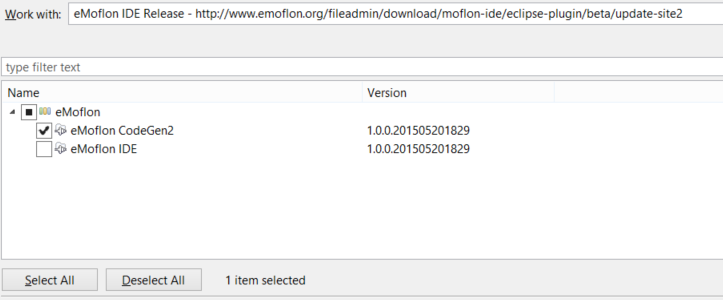
\includegraphics[width=.8\textwidth]{installCodeGen2Feature}
        \caption{Installing the eMoflon CodeGen2 feature}  
        \label{legacyCodegen2:installCodeGen2Feature}
    \end{center}
\end{figure}


\item[$\blacktriangleright$] 
Open the file ``moflon.properties.xmi" in your project(s) and set the code generation strategy to CODEGEN2  (Fig.~\ref{legacyCodegen2:changeCodeGenerationstrategy}).

\begin{figure}[htbp]
    \begin{center} 
        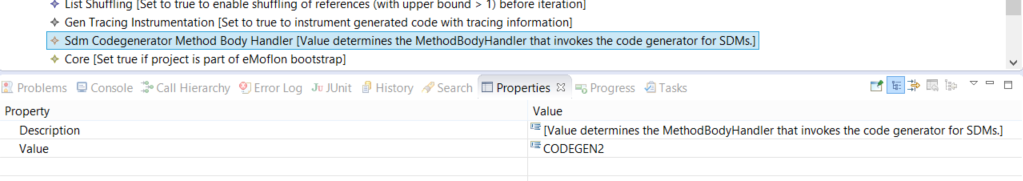
\includegraphics[width=.95\textwidth]{setCodeGenerationStrategy}
        \caption{Code generation strategy selection in ``moflon.properties.xmi"}  
        \label{legacyCodegen2:changeCodeGenerationstrategy}
    \end{center}
\end{figure}


\item[$\blacktriangleright$] 
Open the file ``META-INF/MANIFEST.MF" in your project(s) and add the following dependency: \emph{org.moflon.sdm.codegen2.runtime} (Fig.~\ref{legacyCodegen2:addDependencyToFujabaRuntime}).

\begin{figure}[htbp]
    \begin{center} 
        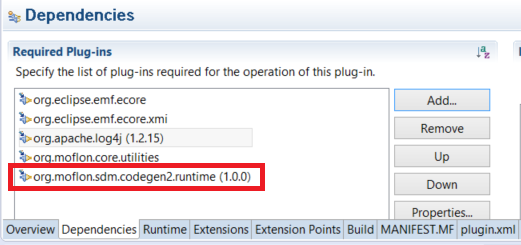
\includegraphics[width=.85\textwidth]{addDependencyToFujabaRuntime}
        \caption{Dependency to CodeGen2 runtime in ``MANIFEST.MF"}  
        \label{legacyCodegen2:addDependencyToFujabaRuntime}
    \end{center}
\end{figure}

\item[$\blacktriangleright$] 
Clean and build your project using the eMoflon context menu (Alt+Shit+E, B).

\end{itemize}
